% !TeX program = xelatex
\documentclass[11pt,a4paper]{ctexart}
\usepackage{amsmath,amssymb}
\usepackage{geometry}
\usepackage{graphicx}
\usepackage{booktabs}
\usepackage{tikz}
% Resolve the schematic when compiling from either the project root or plan/.
\graphicspath{{plan/}{./}}
\geometry{margin=2.4cm}
\setlength{\parindent}{2em}
\setlength{\parskip}{0.25em}
\pagestyle{plain}

\title{基于哑铃形试样平行段等效模型的 DIC--伴随反演实验方案}
\author{}
\date{}

% Historical synthetic figure sources are not present in this checkout.
\newcommand{\historicalfigure}[1]{%
  \IfFileExists{#1}{\includegraphics[width=\linewidth]{#1}}{%
    \fbox{\parbox{0.94\linewidth}{\small 历史合成图件源文件未随当前工作区保存：\par
    {\footnotesize\ttfamily\detokenize{#1}}\par
    本处仅保留原分析文字与统计，不将缺失图件作为本次几何修正的核验证据。}}}%
}

\begin{document}
\maketitle

\noindent\textbf{当前连续七区：}从\texttt{all\_region}提取七个连续16 mm目标区，制造坐标范围$[-56,56]$ mm，总长112 mm；按实际测点截取后为$105.995085\times18.484156$ mm。368$\times$65个DIC参考节点直接用于正反问题，50点L曲线与自由二维反演按新数据重新计算。旧region与粗网格结果分别保留。材料定位沿用已确认共享参考坐标系的原横线位置，既定填充率沿原始$-Y$递增；不根据点云长度重新翻转或居中分区。

\section{实验目的、制造几何与计算范围}
本实验以均匀填充试样标定为独立参照，采用DIC位移识别二维模量$E(x,y)$。比较独立正演、DIC、反演回代及留出载荷预测。每个节点模量独立，不绑定不同$y$行；五区或七区标定仅用于独立正演及后处理，不作为主反演强先验。

已打印哑铃试样总长220 mm，夹持端宽40 mm，厚3.2 mm；平行段长150 mm、宽20 mm。制造坐标$\xi$以试样中心为零、填充率递增为正。原七个制造区为$[-75,-40]$、$[-40,-24]$、$[-24,-8]$、$[-8,8]$、$[8,24]$、$[24,40]$、$[40,75]$ mm，对应40/50/60/70/80/90/100\%；端部制造区各35 mm，中间各16 mm。当前112 mm为连续选域目标，不修改制造几何或打印文件。

\section{全域DIC与连续七区提取}
输入为\texttt{180N\_2/all\_region}、\texttt{280N\_2/all\_region}，各409$\times$65个有效点、15帧，原始跨度约$117.836497\times18.484156$ mm。两者与原\texttt{region}共用初始参考图、毫米坐标原点和方向，已经确认。先恢复参考坐标$X_0=X-DX,Y_0=Y-DY$，保留独立软件毫米标定。

原region两端对应横线，距高填充率外端73 mm、低填充率外端85 mm，其制造坐标为$+37/-25$ mm。原横线中点$Y_0=-21.50749765093$ mm对应$\xi=6$ mm，故沿用
\[
 \xi=-Y_0-15.50749765093\quad\mathrm{mm}.
\]
该映射继承原近似标线中点配准；原region毫米跨度与名义62 mm间隔的0.502646 mm差异仍保留，不重新按大选区边界确定标线。

七个连续16 mm目标区为$\xi\in[-56,56]$ mm。实际全域覆盖$[-50.247810,67.588688]$ mm，40\%端缺5.752190 mm；100\%端保留真实节点边界产生0.252725 mm采样余量。实际截取$[-50.247810,55.747275]$ mm，不补点、不外推、不把七段重新等分。见图~\ref{fig:specimen}。

\begin{figure}[htbp]
\centering
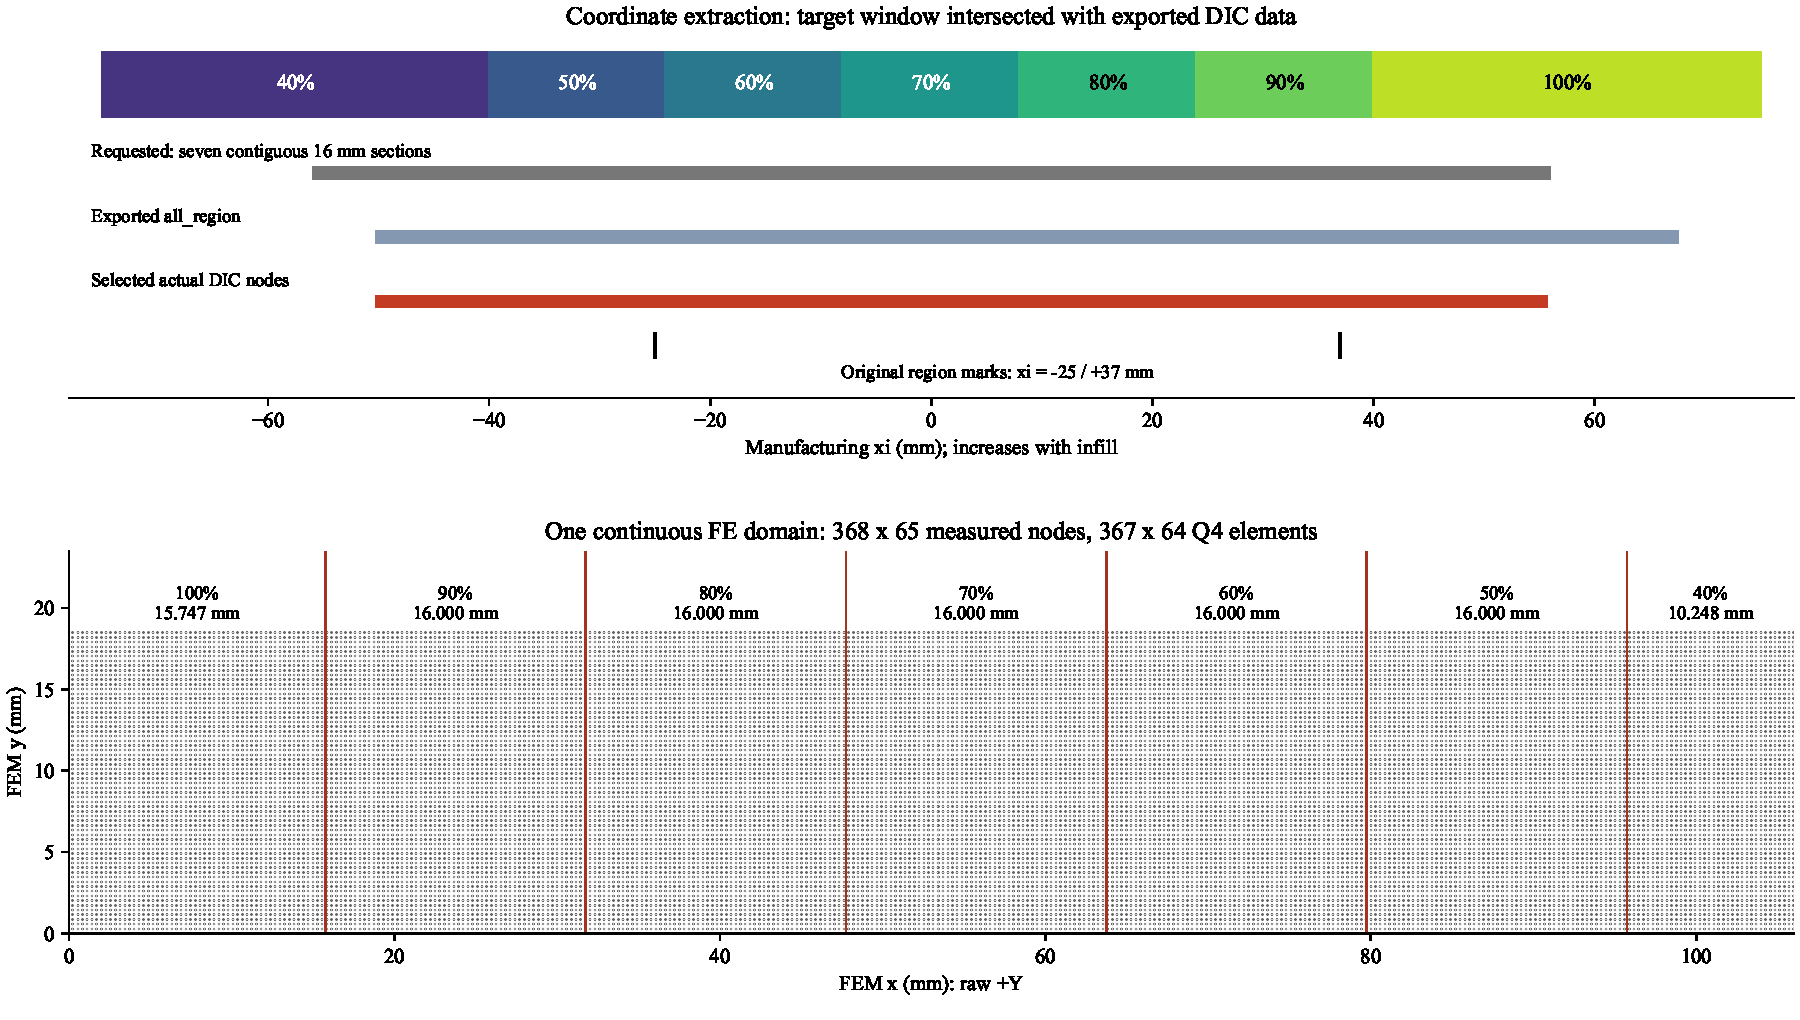
\includegraphics[width=\linewidth]{dic_full_extraction.pdf}
\caption{原制造区、112 mm目标范围、全域导出与实际选取的关系；下图为同一连续DIC节点网格及分区，FEM $x$与制造$\xi$相反。}
\label{fig:specimen}
\end{figure}

当前FEM坐标和位移为
\[
 x=Y_0+71.25477267047,\quad y=-X_0+11.55259777357,
 \qquad u_x=DY,\quad u_y=-DX,
\]
\[
 \xi=55.74727501954-x.
\]
坐标和位移共用正交变换，位置平移不进入位移，不缩放应变。实际沿FEM $x$的分区长度和独立标定如下。

\begin{table}[htbp]
\centering
\caption{实际七区观测覆盖；模量为\texttt{independent}口径，保留批次、样本数与标准差。}
\label{tab:infill}
\begin{tabular}{rrrr}
\toprule
填充率（\%） & FEM $x$范围（mm） & 实际长度（mm） & 标定均值（MPa）\\
\midrule
100 & $[0,15.747275]$ & 15.747275 & 2399.5733\\
90 & $[15.747275,31.747275]$ & 16 & 2120.0569\\
80 & $[31.747275,47.747275]$ & 16 & 1842.0790\\
70 & $[47.747275,63.747275]$ & 16 & 1708.3381\\
60 & $[63.747275,79.747275]$ & 16 & 1638.6619\\
50 & $[79.747275,95.747275]$ & 16 & 1396.4108\\
40 & $[95.747275,105.995085]$ & 10.247810 & 1231.8683\\
\bottomrule
\end{tabular}
\end{table}

在同一完整all\_region网格与观测上只改变材料方向，$\nu=0.26$时180N轴向RMSE由既定方向的5.540变为反向的10.486 $\mu\mathrm m$；280N为9.458与18.809 $\mu\mathrm m$。反向虽使112 mm覆盖差额降至0.411 mm，但覆盖长度不是方向证据，当前响应不支持为截满而翻转。保留既定方向；280N不用于调参，响应对照也不替代独立制造位置核验。

\section{力学边界、观测与二维反演}
当前连续矩形计算域$\Omega=(0,L)\times(0,H)$，其中$L=105.995085$ mm、$H=18.484156$ mm。二维各向同性平面应力采用
\[
 \nabla\cdot\boldsymbol\sigma=\boldsymbol0,\qquad
 \boldsymbol\sigma=\mathsf C(E,\nu):\boldsymbol\varepsilon(\boldsymbol u).
\]
两端牵引$\boldsymbol\sigma\boldsymbol n=\pm q\boldsymbol e_x$，$q=F/(wt)$；真实承载宽$w=20$ mm，厚$t=3.2$ mm。截取域端力$F_{\rm ROI}=FH/w$，单位厚度内核载荷为$F_{\rm ROI}/t$；不能将全部实测力直接作用于较窄ROI。内部横向侧边采用零牵引近似，三个约束只选定刚体规范，不将一端夹紧。坐标、刚体参考、边界等效和实验误差分别评价。

当前网格为367$\times$64个Q4单元、23,920个独立模量参数和47,840个位移自由度。单元约$0.288815\times0.288815$ mm，节点保持实际DIC参考坐标，匹配舍入容限$10^{-7}$ mm。观测$\mathsf H$为节点到测点顺序的双分量置换，不重采样DIC位移。令每个节点$m_a=\log E_a$，
\begin{align}
 E_h(x,y)&=\sum_aN_a(x,y)\exp(m_a),\\
 \min_{\boldsymbol m}\quad &\frac12\sum_k\min_{\boldsymbol c_k}
 \|\mathsf W_k^{1/2}(\mathsf H_k\boldsymbol u(\boldsymbol m;F_k)+\mathsf R_k\boldsymbol c_k-\boldsymbol d_k)\|_2^2
 +\frac\gamma2\int_\Omega|\nabla E_h|^2\,\mathrm dA.
\end{align}
$\mathsf W$仅为测点面积权重，$\mathsf R$只包含两平移及一微小转动；不设参考模量，不作模量或人为噪声尺度归一化。残差配准保留真实伸长、收缩与剪切。独立标定正演在Gauss点使用阶梯材料场，自由反演使用连续节点场。

180N采用259--273帧，实际力119.776179 N；280N采用436--450帧，219.735451 N。60.1 N夹具偏置扣除与初始未加载图参考已确认一致。仅180N、预设主$\nu=0.26$扫描50个对数等距$\gamma\in[10^{-12},10^{-4}]$，按内部正曲率L曲线拐点选择；失败点排除，无可辨识拐点时停止并保留诊断。$\nu=0.24/0.26/0.28/0.33$从同一个所选场出发识别，固定后预测280N，不用留出平台调参。

新选区主$\nu$独立正演的轴向/横向RMSE为180N的4.854/1.643 $\mu\mathrm m$、280N的7.968/3.512 $\mu\mathrm m$。结果位于\texttt{results/dic\_full/}，实际扫描与停止条件见保存记录；函数下降停止、GTOL达标与实验一致性分开报告。新观测域与旧region不同，不仅按绝对RMSE评价扩域优劣。全节点均匀解析误差约$1.32\times10^{-10}$ mm，刚体残差不变性误差约$4.81\times10^{-14}$ mm；实现通过不证明完整狗骨与截取域物理等效。

\section{合成数据先导：全场正则项的形式与边界偏差}
以下保留历史 110 mm 合成研究条件及结果，尚未作为当前 DIC 范围实验验证。该研究在 $55\times10$ 个双线性四边形单元上使用 $616$ 个独立节点模量，令 $m_i=\log E_i$。对两端等大反向的均布牵引及完整节点位移合成观测，实际求解的单载荷目标为
\begin{equation}\label{eq:synthetic_objective}
 J_\gamma(\boldsymbol m)
 =\frac12(\boldsymbol u^{\rm obs}-\boldsymbol u(e^{\boldsymbol m}))^{\mathsf T}
 \mathsf M(\boldsymbol u^{\rm obs}-\boldsymbol u(e^{\boldsymbol m}))
 +\frac{\gamma}{2}\mathcal R(E),\qquad \gamma=10^{-6},
\end{equation}
其中 $\mathsf M$ 为位移的有限元质量矩阵，正问题满足 $\mathsf K(E)\boldsymbol u=\boldsymbol f$ 及三个消除刚体运动的约束。该合成目标尚未包含真实 DIC 测点映射、相关噪声协方差或完整试样肩部的边界误差，不能直接等同于上一节的实验目标。

原始的一阶梯度型 Tikhonov 正则项及本分支新增的\emph{仿射去趋势梯度正则项}分别为
\begin{align}
 \mathcal R_{\rm H1}(E)&=\int_\Omega |\nabla E|^2\,\mathrm dA,
 \\
 \mathcal R_{\rm cgrad}(E)&=\int_\Omega
 \left[(E_x-\overline{E_x})^2+(E_y-\overline{E_y})^2\right]\,\mathrm dA,
 \qquad
 \overline{E_\alpha}=\frac{1}{|\Omega|}\int_\Omega E_\alpha\,\mathrm dA.
\end{align}
这里取的是\emph{全场空间梯度的面积平均}，不是 $E$ 的平均值，也不是事先指定 $E$ 只随 $x$ 变化。将均值展开可得
\begin{equation}\label{eq:regularizer_projection}
 \mathcal R_{\rm cgrad}(E)=\mathcal R_{\rm H1}(E)
 -|\Omega|\left(\overline{E_x}^{\,2}+\overline{E_y}^{\,2}\right).
\end{equation}
这等价于从梯度中正交投影掉全局常斜率分量，仍惩罚其局部变化。任意仿射场 $E=a+bx+cy$ 满足 $\mathcal R_{\rm cgrad}=0$，但反演仍为二维节点场；不应把零惩罚解释成预先指定了实际试样的模量分布。相较之下，$\mathcal R_{\rm H1}$ 也惩罚真实的非零斜率，其单独变分的自然边界条件倾向于零法向斜率，因此可能在截取域端部产生偏置。

离散实现中令 $L_{ij}=\int_\Omega\nabla N_i\!\cdot\!\nabla N_j\,\mathrm dA$、$(g_\alpha)_i=\int_\Omega\partial_\alpha N_i\,\mathrm dA$、$A=|\Omega|$。新增项对节点模量的梯度为
\begin{equation}
 \nabla_{\boldsymbol E}\mathcal R_{\rm cgrad}
 =2\left[L\boldsymbol E-
 \frac{(\boldsymbol g_x^{\mathsf T}\boldsymbol E)\boldsymbol g_x+
       (\boldsymbol g_y^{\mathsf T}\boldsymbol E)\boldsymbol g_y}{A}\right].
\end{equation}
目标函数中的正则项梯度为 $\gamma\nabla_{\boldsymbol E}\mathcal R_{\rm cgrad}/2$；对优化变量 $m_i$ 再乘链式因子 $E_i$，与位移失配项的伴随梯度相加。数值检查包括仿射场零惩罚、正则项有限差分梯度和完整伴随目标对 $\boldsymbol m$ 的有限差分梯度，均已通过。

\subsection{同条件比较与适用边界}
表~\ref{tab:regularization_comparison} 汇总现有合成数据比较。此处代码坐标取 $x\in[0,110]\,\mathrm{mm}$，属于原 110 mm 算例，不能与当前 DIC 范围实验域混用；表中真值表达式的模量单位均为 MPa。相同真值和噪声水平的两种正则项使用同一网格、两端各 $0.01\,\mathrm N$ 的拉力、$t=3.2\,\mathrm{mm}$、初值 $E_i=0.501\,\mathrm{MPa}$、$\gamma=10^{-6}$ 及相同位移观测。左端统计 $x=0\sim10\,\mathrm{mm}$，右端统计 $x=100\sim110\,\mathrm{mm}$；表中指标为节点绝对相对误差的均值（\%）。两种反演均保留 $616$ 个二维节点未知量，表中指数场的真值也只随 $x$ 变化。$1\%$ 噪声行仅是一组随机种子 $42$ 的相同位移噪声样本，不代表跨种子稳定性。

\begin{table}[htbp]
\centering
\small
\caption{原梯度正则项与仿射去趋势正则项的合成数据对比；所有数值单位为绝对相对误差的百分数。}
\label{tab:regularization_comparison}
\begin{tabular}{lllrrr}
\toprule
真值 $E(x)$ & 位移噪声 & 正则项 & 全场 MAE & 左端 MAE & 右端 MAE \\
\midrule
$1+x/110$ & $0$ & $\mathcal R_{\rm H1}$ & 0.2123 & 0.6493 & 0.9571 \\
             &     & $\mathcal R_{\rm cgrad}$ & $8.53\!\times\!10^{-6}$ & $1.67\!\times\!10^{-5}$ & $7.67\!\times\!10^{-6}$ \\
$1+x/110$ & $1\%$ & $\mathcal R_{\rm H1}$ & 1.2050 & 0.6588 & 3.0070 \\
             &        & $\mathcal R_{\rm cgrad}$ & 1.0975 & 0.2550 & 2.3648 \\
$\exp[(\ln2)x/110]$ & $0$ & $\mathcal R_{\rm H1}$ & 0.2256 & 0.4539 & 1.2699 \\
             &     & $\mathcal R_{\rm cgrad}$ & 0.0709 & 0.1846 & 0.3426 \\
$\exp[(\ln2)x/110]$ & $1\%$ & $\mathcal R_{\rm H1}$ & 1.2886 & 0.5118 & 3.3571 \\
             &        & $\mathcal R_{\rm cgrad}$ & 1.2123 & 0.3855 & 2.7145 \\
$\exp[(\ln8)x/110]$ & $0$ & $\mathcal R_{\rm H1}$ & 4.4167 & 1.4291 & 23.7202 \\
             &     & $\mathcal R_{\rm cgrad}$ & 2.7853 & 2.1444 & 14.3102 \\
\bottomrule
\end{tabular}
\end{table}

线性无噪声真值恰好位于 $\mathcal R_{\rm cgrad}$ 的零空间，再加上合成观测与反演使用同一有限元模型，故接近零误差主要证明消除了\emph{该算例的正则化偏置}，不是一般识别精度。原正则项在两端的误差还可通过减小 $\gamma$ 缓和；但先导扫描中 $\gamma=0$ 的二维反演在 $2000$ 次迭代内未收敛，并出现大幅场误差，说明仍需稳定化。新正则项对缓变指数场改善明显，但加入 $1\%$ 噪声后全场收益仅约 $0.076$ 个百分点。对于较陡的 $1\to8\,\mathrm{MPa}$ 指数场，它虽降低全场和右端误差，却使左端误差从 $1.43\%$ 增至 $2.14\%$，且右端仍有 $14.31\%$ 误差。探索性地将该算例的 $\gamma$ 调至 $10^{-8}$ 时，新正则项全场与右端 MAE 分别降至 $0.483\%$ 和 $2.898\%$；该数值是在已知合成真值后查看的，\emph{不能}作为真实实验已验证的选参结果。零噪声小网格上的新正则项 L 曲线各点曾重合、无可辨识拐点，不能机械采用曲率最大规则。

\begin{figure}[htbp]
\centering
\historicalfigure{regularization_linear_field_comparison.pdf}
\caption{线性 $E(x)$、零噪声合成场：上排为两种正则项的二维重建，下排为绝对相对误差；同一行共用色标。新方法接近零误差的前提是线性真值落在其零空间。}
\label{fig:regularization_linear}
\end{figure}

\begin{figure}[htbp]
\centering
\historicalfigure{regularization_exponential_2_field_comparison.pdf}
\caption{缓变指数 $E(x)=\exp[(\ln2)x/110]$、零噪声合成场的同色标比较；新正则项减小两端偏差，但指数曲率仍受到惩罚。}
\label{fig:regularization_exp2}
\end{figure}

\begin{figure}[htbp]
\centering
\historicalfigure{regularization_exponential_8_field_comparison.pdf}
\caption{较陡指数 $E(x)=\exp[(\ln8)x/110]$、零噪声合成场；右端残留的大误差表明，缓变指数算例的改善不能直接外推到高对比度材料。}
\label{fig:regularization_exp8}
\end{figure}

\section{未知真实分布时的正则化策略与初步验证}
真实试样的 $E_{\rm eq}$ 空间形状未知。前述仿射去趋势项来源于已观察到的端部偏差和合成线性真值，它应作为\emph{受控基线}而非默认物理规律。现阶段不宣称存在适用于平滑、指数、七区突变和打印缺陷的单一最优正则项。

\paragraph{低维对照：利用已知制造分区，而不预设模量数值。}
观测域内五区界面位置和填充率顺序来自制造设计；后续可单独构造五参数诊断对照，但当前主流程不采用此参数约束。若在独立对照中使用标定先验，例如
\begin{equation}
 \mathcal R_{\rm cal}(\boldsymbol m)
 =\sum_{i=1}^5\frac{(m_i-m_i^{\rm cal})^2}{(s_i^{\rm cal})^2},
\end{equation}
则不能再把同一标定记录称为该对照的独立验证。标定与分区可能存在工艺差异，应对其不确定度做敏感性分析；五参数对照不能表示区内缺陷、界面扩散或二维变化，也不能取代主二维反演。

\paragraph{需要自由二维场时的候选：二阶总广义变差。}
可测试离散的 Huber 平滑二阶总广义变差（TGV$^2$）型先验\cite{bredies2010tgv}。令 $E_{\rm ref}$ 为独立给定的尺度，并\emph{预先}指定两种候选表示 $z=E/E_{\rm ref}$ 或 $z=\log(E/E_{\rm ref})$，而非观察真实反演结果后再选表示：
\begin{equation}\label{eq:tgv_candidate}
 \mathcal R_{\rm TGV}(z)=\min_{\boldsymbol v}
 \left\{\alpha_1\!\int_\Omega\rho_\delta(|\nabla z-\boldsymbol v|)\,\mathrm dA
 +\alpha_0\!\int_\Omega\rho_\delta(|\operatorname{sym}\nabla\boldsymbol v|)\,\mathrm dA\right\},
\end{equation}
其中 $\rho_\delta(s)=s^2/(2\delta)$（$s\leq\delta$），$\rho_\delta(s)=s-\delta/2$（$s>\delta$）。辅助场 $\boldsymbol v$ 可在平滑区域跟随局部斜率，并允许斜率或模量在少量位置显著改变；它不要求输入线性、指数或七区真值曲线。但两种表示都不是中性的：$z=E/E_{\rm ref}$ 偏好分段仿射模量，$z=\log(E/E_{\rm ref})$ 偏好分段对数仿射模量，后者对应分段指数；两者均可能平滑窄区、移动界面。$\alpha_0,\alpha_1,\delta$ 的选择和带辅助变量的优化均比现有二次项复杂。下文已实现并初步测试 $z=E/E_{\rm ref}$ 的有限元 Huber TGV 型形式；对数表示及真实 DIC 场尚未测试。

若沿用式~\eqref{eq:synthetic_objective} 的位移数据项，拟议的完整优化问题是
\begin{equation}\label{eq:tgv_objective}
 \min_{\boldsymbol m,\boldsymbol v}\;
 \frac12\bigl\|\boldsymbol u^{\rm obs}-\boldsymbol u(e^{\boldsymbol m})\bigr\|_{\mathsf M}^{2}
 +\lambda\!\left[\alpha_1\!\int_\Omega\rho_\delta(|\nabla z(\boldsymbol m)-\boldsymbol v|)\,\mathrm dA
 +\alpha_0\!\int_\Omega\rho_\delta(|\operatorname{sym}\nabla\boldsymbol v|)\,\mathrm dA\right],
\end{equation}
其中 $\|\boldsymbol r\|_{\mathsf M}^2=\boldsymbol r^{\mathsf T}\mathsf M\boldsymbol r$，$\operatorname{sym}\nabla\boldsymbol v=(\nabla\boldsymbol v+\nabla\boldsymbol v^{\mathsf T})/2$。在实测 DIC 上还须将数据项改为有效测点映射与噪声加权形式；此处的 $\lambda$ 控制总强度，$\alpha_0/\alpha_1$ 控制两种变化的相对代价。

\paragraph{与当前一阶梯度型 Tikhonov 的物理解释和数学区别。}
Tikhonov 指 $\|\mathsf Lz\|_2^2$ 一类\emph{二次惩罚}，不是仅能处理光滑场的特定公式；当前代码选择 $\mathsf L=\nabla$，所以 $\mathcal R_{\rm H1}$ 偏好全域常值模量。仿射去趋势项仍是二次梯度惩罚，只是从梯度中移除了\emph{一个全域平均斜率}，偏好全域仿射模量。TGV 型项则用空间变化的 $\boldsymbol v$ 表示\emph{局部}斜率：第一项检查实际梯度是否偏离局部斜率，第二项检查局部斜率变化是否集中在少量位置。其近似线性的大变化代价可允许界面附近出现较陡变化，同时在区内保留平滑斜率；但这仍是统计/结构先验，\emph{不是}额外的弹性本构定律，也不会自动辨认真实填充界面。

一维例子说明差异。对于 $z(x)=a+bx$，一阶梯度平方项为 $b^2L>0$（$b\ne0$）；在式~\eqref{eq:tgv_candidate} 中取 $v=b$，两项均为零。若某一网格宽度 $h$ 内发生幅值 $\Delta z$ 的陡变，一阶梯度平方惩罚约为 $(\Delta z)^2/h$，而 TGV 型第一项在 $|\Delta z|/h\gg\delta$ 时约按 $|\Delta z|$ 增长；因此前者强烈压低和摊宽跳变，后者允许跳变但仍付出代价。对于弯曲的指数场，$z=E/E_{\rm ref}$ 的局部斜率连续改变，TGV 仍有非零惩罚；若选 $z=\log(E/E_{\rm ref})$，纯指数场才是零惩罚。离散网格、Huber 阈值和测量噪声均会影响界面的实际宽度与位置，不能把上述倾向当作反演成功的保证。

\paragraph{避免按已知答案挑选正则项的验证流程。}
先由重复静态 DIC 图像估计测量噪声、空间相关性和有效测点掩膜，在位移数据项中采用相应权重；再用预先固定的线性、缓变/陡变平滑场、七区跳变、混合缺陷及完整试样到截取域的边界失配场景比较 $\mathcal R_{\rm H1}$、$\mathcal R_{\rm cgrad}$、七参数标定约束和式~\eqref{eq:tgv_candidate} 的两种表示。各方法使用相同训练位移、网格、初值规则和计算预算，在独立噪声种子、超过 DIC 噪声相关尺度的留出空间块或重复试样上检查预测位移、端部/界面误差、模量不确定度及收敛失败率；合成真值仅用于\emph{最后}的误差评估，不用于挑选该测试样本的 $\gamma$。留出位移预测正确也不保证模量唯一，仍需独立模量标定和参数灵敏度检查。载荷级在线弹性区内基本按比例缩放，可改善信噪比，但不能单独增加新的空间灵敏度。只有跨场景、跨噪声和边界扰动仍有收益时，才将更复杂的先验用于实测数据；正则化不能代替对牵引边界误差的检验。

\subsection{二维 Huber TGV 型正则项的实现与受控测试}
实际实现先按几何和模量尺度无量纲化：$\boldsymbol\xi=(x,y)/\ell$、$\ell=20\,\mathrm{mm}$、$z=E/(1\,\mathrm{MPa})$，并固定 $r=2$、$\delta=0.02$。本次求解的正则项及总目标为
\begin{align}
 \mathcal R_{\rm TGV,h}(E,\boldsymbol v)
 &=\int_{\Omega/\ell}\left[\rho_\delta(|\nabla_{\boldsymbol\xi}z-\boldsymbol v|)
 +r\rho_\delta(|\operatorname{sym}\nabla_{\boldsymbol\xi}\boldsymbol v|_{\rm F})\right]\,\mathrm d\boldsymbol\xi,
 \\
 \min_{\boldsymbol m,\boldsymbol v}\ J_\gamma
 &=\tfrac12\|\boldsymbol u^{\rm obs}-\boldsymbol u(e^{\boldsymbol m})\|_{\mathsf M}^2
 +\tfrac\gamma2\mathcal R_{\rm TGV,h}(e^{\boldsymbol m},\boldsymbol v).
\end{align}
积分换元包含 $\mathrm d\boldsymbol\xi=\mathrm dA/\ell^2$，微分换元为 $\nabla_{\boldsymbol\xi}=\ell\nabla_{x,y}$。模量和辅助向量场均用连续双线性有限元插值、$2\times2$ Gauss 积分；张量采用 Frobenius 范数，包含两个对称剪切分量的贡献。仍保留 $616$ 个独立二维节点模量，并额外优化 $1232$ 个局部斜率自由度。优化变量使用 $m=\log E$ 保证正值，但正则项作用于 $E$。连续节点模量只能用至少一个单元宽度表示陡变，因此这是有限维、Huber 平滑的 TGV 型近似。完整目标对全部模量和辅助变量的有限差分梯度检查，以及任意二维仿射场的零惩罚检查均已通过。

\paragraph{固定协议与不依赖模量真值的选参。}
采用相同的 $55\times10$ 网格、双端载荷和 $E_i=0.501\,\mathrm{MPa}$ 初值，分别测试线性 $1+x/110$、指数 $\exp[(\ln2)x/110]$，以及等宽七段模量 $[1,1.4,1.2,1.8,1.5,2,1.7]\,\mathrm{MPa}$。七段算例仍在矩形域上，不代表已测试实际狗骨七区几何。所有位移使用现有逐分量、相对幅度 $1\%$ 的独立 Gaussian 噪声模型。先用种子 $40$ 的位移拟合，在 $\gamma\in\{10^{-7},10^{-6},10^{-5}\}$ 中，按另一份独立重复观测（种子 $1040$）的质量矩阵加权位移误差为每种方法选参。随后固定参数，以测试种子 $42,43,44$ 从相同初值重新反演，最后才用模量真值评分。每次均最多 $2000$ 次迭代、约 $2400$ 次目标计算；Huber 阈值与两项相对权重未按最终误差调节。

\begin{table}[htbp]
\centering
\small
\caption{独立重复位移选参后，三个测试噪声种子的平均结果。误差单位为 \%；耗时为当前机器单次反演的平均秒数，不含选参扫描。}
\label{tab:tgv_results}
\begin{tabular}{llrrrr}
\toprule
真值 & 正则项 & 所选 $\gamma$ & 全场 MAE & 右端 MAE & 耗时（s） \\
\midrule
线性 & 梯度 Tikhonov & $10^{-6}$ & 1.2208 & 2.5304 & 5.70 \\
 & 仿射去趋势 & $10^{-5}$ & 0.4727 & 0.8372 & 3.33 \\
 & Huber TGV & $10^{-5}$ & 0.2812 & 0.7673 & 12.47 \\
指数 & 梯度 Tikhonov & $10^{-6}$ & 1.3119 & 2.8249 & 6.12 \\
 & 仿射去趋势 & $10^{-5}$ & 0.5707 & 1.2914 & 3.32 \\
 & Huber TGV & $10^{-5}$ & 0.6590 & 2.4324 & 13.26 \\
七段 & 梯度 Tikhonov & $10^{-7}$ & 5.1683 & 6.1890 & 11.47 \\
 & 仿射去趋势 & $10^{-7}$ & 5.1727 & 6.1453 & 11.61 \\
 & Huber TGV & $10^{-6}$ & 3.3053 & 3.5779 & 34.12 \\
\bottomrule
\end{tabular}
\end{table}

\paragraph{收益、反例与计算代价。}
七段场中，TGV 相对原梯度项的平均全场误差下降约 $36.0\%$，三个测试种子均改善；区内平台更平坦，但部分幅值仍有收缩，最大节点误差仍为 $17.1\%\sim23.9\%$，并未精确恢复界面。线性场的 TGV 全场误差范围为 $0.234\%\sim0.372\%$，低于本次仿射去趋势的 $0.362\%\sim0.581\%$。指数场则构成反例：TGV 的平均全场及右端误差均高于仿射去趋势，左端也由 $0.479\%$ 增至 $0.946\%$；TGV 三种子的全场范围为 $0.420\%\sim0.874\%$。局部斜率变化的惩罚可能压制真实曲率，与端部误差相符，但尚未通过独立消融定量分解原因。最终 $27$ 次测试均取得 SciPy 成功状态；TGV 七段场耗费 $1999,1839,1833$ 次迭代，明显多于二次项约 $600$ 次。校准阶段 $\gamma=10^{-7}$ 的三个 TGV 候选均耗尽预算，且均未被选中，失败日志保留。

\paragraph{结论的范围。}
这只是\emph{预设参数范围内}的初步比较，不能把上表当作各方法最优性能：部分方法选择到扫描边界，而且指数场 TGV 在 $10^{-6}$ 与 $10^{-5}$ 时的验证位移代价仅相差约 $0.081\%$，一次重复观测不足以稳定区分。位移预测较好不保证模量误差较小，故没有按测试模量误差重新选参。当前证据支持保留 TGV 作为分区材料候选，\emph{不支持全面替换}仿射去趋势默认项；后续若扩大参数范围或改变表示，应使用新的预先固定测试数据。相关噪声、完整试样边界失配、真实七区几何和 $\log E$ 表示均未在本次验证。可复现脚本为 \texttt{script/benchmark\_tgv\_regularization.py}，原始数组、参数记录、收敛日志和全部二维场图保存在独立的 \texttt{results/tgv\_comparison\_20261015/} 目录。

\begin{figure}[htbp]
\centering
\historicalfigure{tgv_20261015_linear_fields.pdf}
\caption{线性真值、$1\%$ 位移噪声、预先指定的测试种子 $42$：真值与三种方法的二维模量及误差场，同一行共用色标。图中为单个种子，表~\ref{tab:tgv_results} 为三种子平均。}
\end{figure}
\begin{figure}[htbp]
\centering
\historicalfigure{tgv_20261015_exponential_fields.pdf}
\caption{指数真值的相同协议比较。TGV 减少区内噪声，但本次两端精度不及仿射去趋势；这限制了由线性场推断其一般优势的结论。}
\end{figure}
\begin{figure}[htbp]
\centering
\historicalfigure{tgv_20261015_layered_fields.pdf}
\caption{七段升降跳变真值的相同协议比较。TGV 改善平台并降低平均误差，界面仍有明显局部误差；本图是矩形合成场，未引入真实狗骨肩部与分区界面误差。}
\end{figure}

\newpage
\section{等效模型的验证与结果判据}
先用同一打印参数制备各填充率均匀试样，独立获得等效模量参考值。随后对分区试样进行重复拉伸试验，比较反演模量、独立标定值以及由标定值正向预测的 DIC 位移场。报告分区误差、重复性、位移残差与载荷级敏感性；不同载荷级应保持在线弹性范围内。

在解释实验结果前，对两种分区分别进行完整试样与截取矩形模型的配对计算：在完整模型中施加实际夹持条件，提取 $\Omega$ 端部的法向、切向牵引及域内位移，再检验均布牵引矩形模型造成的位移和模量偏差。方案 B 还应依据 DIC 噪声水平检查各 $E_i$ 的位移灵敏度及参数相关性。只有当边界近似偏差和反演误差均低于预设容许值时，才使用均布牵引矩形模型解释相应实验；否则应调整加载与边界建模，或保留完整试样模型。

\begin{thebibliography}{9}
\bibitem{bredies2010tgv}
K.~Bredies, K.~Kunisch, and T.~Pock,
``Total generalized variation,''
\emph{SIAM Journal on Imaging Sciences}, vol.~3, no.~3, pp.~492--526, 2010.
doi:10.1137/090769521.
\end{thebibliography}

\end{document}
